\section{Prompts and Datasets}

\subsection{Prompts for Conversation}\label{ss:prompts}

\textsc{\textbf{Two Professors}}


% \texttt{Convert the context above as a multi-turn discussions between two professors. Make sure that their discussions strictly adhere to the context above and remains faithful to information in the context. Please DONOT add any new information/reference other than the context.}
\begin{tcolorbox}[colback=blue!5!white,colframe=white]
  Convert the context above as a multi-turn discussions between two professors. Make sure that their discussions strictly adhere to the context above and remains faithful to information in the context. Please DONOT add any new information/reference other than the context.
\end{tcolorbox}


\textsc{\textbf{Teacher Student}}

% \texttt{Convert the context above as a multi-turn discussions between a teacher and a student. The student has questions about the context and the teacher solves each of them step-by-step. Make sure that their discussions strictly adhere to the context above and remains faithful to information in the context. Please DONOT add any new information/reference other than the context.}

\begin{tcolorbox}[colback=blue!5!white,colframe=white]
  Convert the context above as a multi-turn discussions between a teacher and a student. The student has questions about the context and the teacher solves each of them step-by-step. Make sure that their discussions strictly adhere to the context above and remains faithful to information in the context. Please DONOT add any new information/reference other than the context.
\end{tcolorbox}


\textsc{\textbf{Two Students}}

% \texttt{Convert the context above as a multi-turn discussions between two students who are working on their assignment related to the given context. Make sure that their discussions strictly adhere to the context above and remains faithful to information in the context. Please DONOT add any new information/reference other than the context.}
\begin{tcolorbox}[colback=blue!5!white,colframe=white]
  Convert the context above as a multi-turn discussions between two students who are working on their assignment related to the given context. Make sure that their discussions strictly adhere to the context above and remains faithful to information in the context. Please DONOT add any new information/reference other than the context.
\end{tcolorbox}


\textsc{\textbf{Interview}}

% \texttt{Conduct an interview-style conversation where one participant acts as the interviewer, asking questions exclusively related to the content provided, while the other participant serves as the subject matter expert, providing detailed responses based on the content. Make sure that their discussions strictly adhere to the context above and remains faithful to information in the context. Please DONOT add any new information/reference other than the context.}
\begin{tcolorbox}[colback=blue!5!white,colframe=white]
  Conduct an interview-style conversation where one participant acts as the interviewer, asking questions exclusively related to the content provided, while the other participant serves as the subject matter expert, providing detailed responses based on the content. Make sure that their discussions strictly adhere to the context above and remains faithful to information in the context. Please DONOT add any new information/reference other than the context.
\end{tcolorbox}

\textsc{\textbf{Problem Solving}}

% \texttt{Convert the context above as a multi-turn problem-solving conversation where participants analyze challenges or scenarios presented in the content and brainstorm solutions within the context of the provided material, avoiding speculation or unrelated discussions. Make sure that their conversation strictly adhere to the context above and remains faithful to information in the context. Please DONOT add any new information/reference other than the context.}

\begin{tcolorbox}[colback=blue!5!white,colframe=white]
  Convert the context above as a multi-turn problem-solving conversation where participants analyze challenges or scenarios presented in the content and brainstorm solutions within the context of the provided material, avoiding speculation or unrelated discussions. Make sure that their conversation strictly adhere to the context above and remains faithful to information in the context. Please DONOT add any new information/reference other than the context.
\end{tcolorbox}


\textsc{\textbf{Layman Know-All}}

\begin{tcolorbox}[colback=blue!5!white,colframe=white]
  Imagine you are presenting the content above step-by-step to a layman. While you are presenting, the layman has a lot of followup questions regarding your presentation. You answer the questions step-by-step with chain-of-thoughts. Design this interaction between you and the layman as a multi-turn conversational manner. Make sure that the interaction strictly adhere to the context above and remains faithful to information in the context. Please DONOT add any new information/reference other than the context.
\end{tcolorbox}

% \texttt{Imagine you are presenting the content above step-by-step to a layman. While you are presenting, the layman has a lot of followup questions regarding your presentation. You answer the questions step-by-step with chain-of-thoughts. Design this interaction between you and the layman as a multi-turn conversational manner. Make sure that the interaction strictly adhere to the context above and remains faithful to information in the context. Please DONOT add any new information/reference other than the context.}

\textsc{\textbf{Debate}}

% \noindent\fbox{%
%     \parbox{\textwidth}{%
%         Convert the context above as a multi-turn debate-style conversation where the participants present arguments and counterarguments based solely on the content provided, without introducing external information or personal opinions. Each participant defends others arguments step-by-step with chain-of-thoughts. Make sure that the conversation strictly adhere to the context above and remains faithful to information in the context. Please DONOT add any new information/reference other than the context.
%     }%
% }

% \begin{tcolorbox}[width=\textwidth,colback={yellow},title={With rounded corners},colbacktitle=yellow,coltitle=black]    
%    \blindtext[1]
% \end{tcolorbox}
% \texttt{Convert the context above as a multi-turn debate-style conversation where the participants present arguments and counterarguments based solely on the content provided, without introducing external information or personal opinions. Each participant defends others arguments step-by-step with chain-of-thoughts. Make sure that the conversation strictly adhere to the context above and remains faithful to information in the context. Please DONOT add any new information/reference other than the context.}


\begin{tcolorbox}[colback=blue!5!white,colframe=white]
  Convert the context above as a multi-turn debate-style conversation where the participants present arguments and counterarguments based solely on the content provided, without introducing external information or personal opinions. Each participant defends others arguments step-by-step with chain-of-thoughts. Make sure that the conversation strictly adhere to the context above and remains faithful to information in the context. Please DONOT add any new information/reference other than the context.
\end{tcolorbox}


\subsection{Evaluation Metric Details}

We evaluate the \llm trained on raw and synthetic data using ten diverse general reasoning tasks, three mathematical tasks and one specialized knowledge tasks. 

\paragraph{General Purpose Reasoning Tasks.} All the benchmarks under this category are evaluated in zero-shot manner.
\begin{itemize}[leftmargin=*]
    \item \textbf{ARC Easy (ARC-E) and ARC Challenge (ARC-C)} \citep{clark2018thinksolvedquestionanswering}: This dataset is proposed by the AI2 Reasoning Challenge (ARC). There are two sets of this data: (1) ARC-E and (2) ARC-C, containing science exam questions from grades 3 to 9. The ARC Challenge set includes more difficult questions compared to ARC-E that necessitate higher-order reasoning.
    \item \textbf{RACE} \citep{lai-etal-2017-race}: This dataset has been collected from English reading comprehension exams designed for middle and high school Chinese students. 
    \item \textbf{PIQA} \citep{bisk2020piqa}: Physical Interaction Question Answering evaluates physical commonsense reasoning ability of the language model.
    \item \textbf{Winogrande} [Wino.]\citep{sakaguchi2019winogrande}: This benchmark is structured as a fill-in-the-blank task with binary options, requiring the \llm to select the correct option for a given sentence, primarily focusing on commonsense reasoning and pronoun disambiguation tasks.
    \item \textbf{HellaSwag} \citep{zellers2019hellaswag}: This dataset evaluates a model's ability to resolve scenarios in a way that is both contextually appropriate and logically consistent, testing its grasp of language comprehension and commonsense reasoning.
    \item \textbf{OpenBookQA} [OBQA]\citep{OpenBookQA2018}: This dataset is designed to evaluate deeper understanding of elementary science facts by requiring models to apply these facts to novel situations using both open book knowledge and external commonsense reasoning.
    \item \textbf{TruthfulQA} [TFQA] \citep{lin-etal-2022-truthfulqa}: Evaluates models' ability to generate factually correct answers by presenting 817 questions across 38 categories, designed to challenge common misconceptions.
    \item \textbf{CommonSenseQA} [CSQA] \citep{talmor-etal-2019-commonsenseqa}: This dataset has been designed to test commonsense reasoning through multiple-choice questions created from \textsc{ConceptNet} \citep{speer2017conceptnet} relations, which requires prior knowledge beyond contextual associations for accurate answering.
    \item \textbf{Social-IQA} [SIQA] \citep{sap-etal-2019-social}: Evaluates \llm's ability to reason about people’s actions and their social implications.
\end{itemize}

\paragraph{Math and Specialized Knowledge Tasks.} For these tasks, we evaluate the \llm in few-shot manner.
\begin{itemize}[leftmargin=*]
    \item \textbf{\gsm} \citep{cobbe2021gsm8k}: This benchmark comprises of high quality linguistically diverse grade school math word problems that evaluates the multi-step and logical reasoning ability of \llm. In this setup, we prompt the \llm with eight chain-of-thought examples from \cite{wei2022chain} and take the majority vote of the answers from greedy decoding following the approach in \cite{wang2022self}.
    \item \textbf{\mathall} \citep{hendrycksmath2021}: This dataset contains challenging competition mathematics problems that requires step-by-step processing of the problem to derive the solution. We choose 4-shot prompt from \cite{lewkowycz2022solving} for our evaluation process.
        \item \textbf{\mmlu} \citep{hendryckstest2021}: This task is designed to evaluate a \llm's multitask accuracy across 57 diverse subjects, including elementary mathematics, US history, and law in multiple-choice question format, requiring extensive world knowledge and problem-solving skills for high performance. We explicitly consider \mmlus as it contains comprehensive math and science problems that requires multi-hop and complex reasoning ability. Using the evaluation pipeline of LM Eval Harness, we evaluate the \llm with 5-shot prompts for this task. 
\end{itemize}


\section{Additional Experiments and Results}
\subsection{Results of Pretraining \llm from Scratch}\label{ss:pt_results}

We pretrain a 8B \llm from scratch with 300B tokens using (i) 4 snapshots of \cc (ii) \owma-4B and (iii) wikipedia, books and epubs corpus corresponding to 486B, 4B and 84B original tokens respectively. To emphasize math over other datasets, we provide 8 epochs of \owma-4B in the pretraining blend resulting in 35B \owma tokens that will be seen by the \llm during pretraining. For all other datasets, we maintain 0.46 epochs. For our experimentation with synthetic corpus, we analyze four variations in the \owma corpus while keeping the other data constant:  

\begin{itemize}[leftmargin=*] 
\item \textbf{\ourdata-4B [\tss].} This data includes conversations between two students. 
\item \textbf{\owma-4B + \ourdata-4B [1:1].} We sample raw and synthetic conversations in a 1:1 ratio, ensuring an equal number of tokens to be seen during pretraining from both sources. For the synthetic data, we utilize the \tss conversations. 
\item \textbf{\owma-4B + \ourdata-4B [Concat].} We concatenate each raw context with all seven synthetic conversations sequentially. 
\item \textbf{\ourdata-4B [Longest Conversation].} From the seven conversations generated for each context, we select the longest conversation in token count. 
\end{itemize}

\begin{table*}[ht]
\begin{center}
\resizebox{\textwidth}{!}{% 
\begin{tabular}{@{}lccccccccccc@{}}
\toprule
\textbf{Dataset} & \textbf{ARC-E}        & \textbf{Race} & \textbf{PIQA} & \textbf{Wino.} & \textbf{HellaSwag} & \textbf{ARC-C} & \textbf{OBQA} & \textbf{TFQA} & \textbf{CSQA}& \textbf{SIQA} & \textbf{Avg-All}\\\toprule
\owma-4B & 66.79	&35.98	&77.69	&62.19	&68.23	&38.91	&37.20	&35.92	&19.57	&44.42	&48.69\\ \midrule
\ourdata-4B [\tss] & 68.14	&36.75	&77.86	&63.06	&69.11	&40.19&	39.40	&37.80	&19.66	&45.55	&49.75 \\
\owma-4B+\ourdata-4B [1:1] & 69.74	&37.32	&77.64	&63.69	&69.51	&40.87	&38.20	&34.97	&20.39	&44.47	&49.68\\
\owma-4B+\ourdata-4B [Concat] & 69.28&	38.37	&78.02	&64.09	&68.66	&39.76&	39.00	&38.38	&22.52	&44.63	&50.27\\
\ourdata-4B [Longest Conversation] & 68.39	&36.75&	77.64	&62.04	&68.91	&40.02&	39.40	&38.23	&20.23	&44.52&	49.61\\
\toprule
\end{tabular}
}
\end{center}
\caption{\textbf{Evaluation of 8B \llm on General Reasoning tasks:} Conversations provide improvement over raw data in general purpose reasoning tasks including commonsense, factual and social reasoning tasks.}
\label{tab:8b_pt_non_mmlu}
\end{table*}

As shown in \autoref{tab:8b_pt_non_mmlu}, conversational synthetic data improves general purpose reasoning ability of \llm. Specifically, the concatenation of raw text and conversations yields the best average score for all combinations---highlighting the efficacy of both data towards generalizability of \llm across wide range of reasoning tasks.


\begin{table*}[ht!]
\begin{center}
\resizebox{\textwidth}{!}{% 
\begin{tabular}{@{}lcccccccc@{}}
\toprule
\textbf{Dataset} &	\textbf{GSM8K} &	\textbf{MATH}	& \textbf{\shortstack{MMLU-\\STEM}} &\textbf{\shortstack{MMLU-\\Humanities}}	& \textbf{\shortstack{MMLU-\\Social-Sciences}}	& \textbf{\shortstack{MMLU-\\Others}} & \textbf{MMLU} & \textbf{Avg-All}\\\toprule
\owma-4B &  4.78	&4.92&	26.29&	25.93&	26.75	&27.16	&26.46&	12.05  \\\midrule
% \owma-14B &  70.88	& 38.76 &	78.78 &	67.80 & 73.90 & 43.86 & 42.60 & 41.35 & 29.65 & 44.63 & 53.22 \\\midrule
\ourdata-4B [\tss] & 10.77&	5.30&	26.93&	26.78	&26.81&	27.87&	27.06&	14.38 \\
\owma-4B+\ourdata-4B [1:1] & 8.49	&5.02	&28.01	&28.44&	28.40&	28.39&	28.32&	13.94\\ 
\owma-4B+\ourdata-4B [Concat] & 8.04	&4.98	&29.18	&29.22	&29.51	&31.54	&29.79	&14.27 \\
\ourdata-4B [Longest Conversation] & 8.57	&4.60	&26.77	&27.16	&29.12	&29.29	&27.97	&13.71\\
\toprule
\end{tabular}
}
\end{center}
\caption{\textbf{Evaluation of 8B \llm on Math and Specialized Knowledge tasks:} Conversations are always beneficial for mathematical reasoning where specialized knowledge tasks further benefit from having both raw and synthetic data in the corpus.}
\label{tab:8b_pt_mmlu}
\end{table*}

In addition, for mathematical benchmarks, only synthetic data produce the best imrpovement over the raw data (\autoref{tab:8b_pt_mmlu}). The nature of conversational data being composite and structured helps the \llm to perform well in tasks that requires step-by-step processing of a complex problem. Conversely, specialized knowledge tasks require both raw and synthetic data to attain the maximum gain.

\subsection{Breakdown of Individual Tasks Results of Continued Pretrained \llm}\label{ss:break_tasks}

In this section, we further breakdown the performance of models trained on individual and combinations of conversation styles across general purpose reasoning tasks and specialized knowledge tasks. 

\paragraph{Performance across Individual Prompt Style.} As shown in \autoref{tab:7b_break_non_mmlu}, synthetic data overall achieves highest gain for general purpose reasoning task compared to using raw or rephrased data. \autoref{tab:7b_break_mmlu} further validates the efficacy of synthetic conversations on mathematical reasoning tasks where model trained with all styles of conversational data generated from \owma-4B gets the highest gain across all other models---highlighting the potential of upsampling high-quality data by generating synthetic data of diverse styles using a small seed data.

% \begin{table*}[ht]
% \begin{center}
% \resizebox{\textwidth}{!}{% 
% \begin{tabular}{@{}lcccccccccccc@{}}
% \toprule
% \textbf{Dataset} & \textbf{Style} & \textbf{ARC-E}        & \textbf{Race} & \textbf{PIQA} & \textbf{Wino.} & \textbf{HellaSwag} & \textbf{ARC-C} & \textbf{OBQA} & \textbf{TFQA} & \textbf{CSQA} & \textbf{SIQA} & \textbf{Avg-All}\\\toprule
% \owma-4B &   Raw & 71.89   & 37.89 & 78.24 &  65.98 & 71.42 & 46.33	& 41.40	& 36.96 & 32.35 & 46.57 & 52.90\\ \midrule
% % & \mawps           & \textbf{69.83}         & 66.83            \\ 
% \multirow{7}{*}{\ourdata-4B} & \tp & 72.18	&38.85	&77.20	&66.38	&71.54	&44.20	&40.40	&42.51	&32.35	&46.47  & -\\ 
%  & \ts & 75.17&	38.76	&78.35&	66.46	&72.08	&47.70	&40.20	&44.88	&38.74	&46.06  &-\\ 
% & \tss & 72.90&	38.56&	78.24	&65.82	&72.24	&46.67	&41.00	&44.10	&38.25	&45.45 & -\\  
% & \lk & 74.12	& 39.04 &	78.45 &	65.27 &	72.19 & 46.42 & 41.00 & 46.25 & 41.28	& 44.88 & -\\
% & \deb & 74.92	& 38.37 &	78.45 &	65.75 &	71.89 & 47.78 & 40.40 & 45.47 & 38.41	& 46.16 & -\\
% & \intr & 73.82	& 37.99 &	78.13 &	65.11 &	72.18 & 48.72 & 42.00 & 47.81 & 36.04	& 45.45 & -\\
% & \ps & 74.41	& 38.37 &	78.07 &	65.59 &	71.67 & 49.40 & 41.20 & 47.04 & 37.02	& 46.26 & -\\ \cmidrule{2-13}
% & \textsc{Longest Conversation} & 74.71&	37.99	&78.18	&64.80	&72.10	&47.61	&41.40	&45.49&	39.80&	46.52& 54.86\\ 
% \toprule
% \end{tabular}
% }
% \end{center}
% \caption{\textbf{Results of 7B \llm on General Reasoning Tasks:} We evaluate both the baseline and model trained with synthetic data across diverse tasks that focus on general reasoning, language understanding and commonsense.}
% \label{tab:8b_cont_non_mmlu}
% \end{table*}








\begin{table*}[ht]
\begin{center}
\resizebox{\textwidth}{!}{% 
\begin{tabular}{@{}lcccccccccccc@{}}
\toprule
\textbf{Dataset} & \textbf{Style} & \textbf{ARC-E}        & \textbf{Race} & \textbf{PIQA} & \textbf{Wino.} & \textbf{HellaSwag} & \textbf{ARC-C} & \textbf{OBQA} & \textbf{TFQA} & \textbf{CSQA} & \textbf{SIQA} & \textbf{Avg-All}\\\toprule
\owma-4B &   Raw & 71.89   & 37.89 & 78.24 &  65.98 & 71.42 & 46.33	& 41.40	& 36.96 & 32.35 & 46.57 & 52.90\\ \midrule
Rephrase-\owma-4B &  Rephrase &72.05	&38.28	&78.07	&63.14	&71.16&	45.31	&42.20	&47.09	&33.33	&45.19 & 53.58 \\\midrule
% & \mawps           & \textbf{69.83}         & 66.83            \\ 
\multirow{9}{*}{\ourdata-4B} & \tp & 72.18	&38.85	&77.20	&66.38	&71.54	&44.20	&40.40	&42.51	&32.35	&46.47  & 53.21\\ 
 & \ts & 75.17&	38.76	&78.35&	66.46	&72.08	&47.70	&40.20	&44.88	&38.74	&46.06  & 54.84\\ 
& \tss & 72.90&	38.56&	78.24	&65.82	&72.24	&46.67	&41.00	&44.10	&38.25	&45.45 & 54.32\\  
& \lk & 74.12	& 39.04 &	78.45 &	65.27 &	72.19 & 46.42 & 41.00 & 46.25 & 41.28	& 44.88 & 54.89\\
& \deb & 74.92	& 38.37 &	78.45 &	65.75 &	71.89 & 47.78 & 40.40 & 45.47 & 38.41	& 46.16 & 54.76\\
& \intr & 73.82	& 37.99 &	78.13 &	65.11 &	72.18 & 48.72 & 42.00 & 47.81 & 36.04	& 45.45 & 54.73\\
& \ps & 74.41	& 38.37 &	78.07 &	65.59 &	71.67 & 49.40 & 41.20 & 47.04 & 37.02	& 46.26 & 54.90\\ \cmidrule{2-13}
& \textsc{Longest Conversation} & 74.71&	37.99	&78.18	&64.80	&72.10	&47.61	&41.40	&45.49&	39.80&	46.52& 54.86\\ 
& \textsc{All Conversations} & 75.17 & 39.04 & 77.86 & 65.43 & 72.31 & 49.40 &	41.00 &	46.68 &	40.79 &	46.42 & 55.41\\\midrule
\owma-4B+\ourdata-4B [1:1] & \multirow{2}{*}{Combination} & 74.12 & 37.99 & 78.18 & 66.54 & 72.28 & 48.12 &	41.40 &	39.27 &	40.70 &	46.37 & 54.50\\ 
\owma-4B+\ourdata-4B [Concat] & & 74.92 & 38.28 & 77.58 & 67.32 & 72.63 & 48.55 &	41.80 &	42.26 &	40.95 &	46.72 & 55.10\\
\toprule
\end{tabular}
}
\end{center}
\caption{\textbf{Results of 7B \llm on General Reasoning Tasks:} We evaluate both the baseline and model trained with synthetic data across diverse tasks that focus on general reasoning, language understanding and commonsense.}
\label{tab:7b_break_non_mmlu}
\end{table*}


% \begin{table*}[ht]
% \begin{center}
% \resizebox{\textwidth}{!}{% 
% \begin{tabular}{@{}lccccccccc@{}}
% \toprule
% \textbf{Dataset} & \textbf{Style} & \textbf{GSM8K} &	\textbf{MATH}	& \textbf{\shortstack{MMLU-\\STEM}} &\textbf{\shortstack{MMLU-\\Humanities}}	& \textbf{\shortstack{MMLU-\\Social-Sciences}}	& \textbf{\shortstack{MMLU-\\Others}} & \textbf{MMLU} & \textbf{Avg-All}\\\toprule
% \owma-4B &   Raw & 12.96 & 4.92 & 39.39 & 41.15 & 52.84 & 52.85 & 45.91 & 35.72\\ \midrule
% % & \mawps           & \textbf{69.83}         & 66.83            \\ 
% \multirow{7}{*}{\ourdata-4B} & \tp & 13.50 & 4.52 & 37.93 & 41.89 & 52.32 & 50.76 & 45.25 & 35.17\\ 
%  & \ts & 22.74 & 5.96 & 40.72 & 42.21 & 56.78 & 55.13 & 47.93 & 38.78\\ 
% & \tss & 21.30 & 6.20 & 41.90 & 43.40 & 57.07 & 55.65 & 48.77 & 39.18\\  
% & \lk & 17.74 & 5.46 & 41.96 & 44.27 & 56.19 & 55.62 & 48.87 & 38.59\\
% & \deb & 23.96 & 6.12 & 40.18 & 42.40 & 55.38 & 55.33 & 47.61 & 38.71\\
% & \intr & 20.92 & 5.86 & 40.53 & 41.21 & 55.48 & 53.91 & 46.99 & 37.84\\
% & \ps & 24.72 & 6.16 & 41.36 & 42.21 & 55.18 & 55.23 & 47.74 & 38.94\\ \cmidrule{2-10}
% & \textsc{Longest Conversation} & 25.78 & 6.30 & 42.72 & 43.53 & 57.52 & 56.90 & 49.37 & 40.30\\
% \toprule
% \end{tabular}
% }
% \end{center}
% \caption{\textbf{Results of 7B \llm on Specialized Knowledge Tasks:} In this setup, we assess the domain specific knowledge of \llm specifically on mathematics, science and general knowledge. We emphasize on the GSM8K, MATH and MMLU-STEM task, as these tasks  predominantly checks the mathematical reasoning ability of the \llm.}
% \label{tab:8b_cont_mmlu}
% \end{table*}













\begin{table*}[ht]
\begin{center}
\resizebox{\textwidth}{!}{% 
\begin{tabular}{@{}lccccccccc@{}}
\toprule
\textbf{Dataset} & \textbf{Style} & \textbf{GSM8K} &	\textbf{MATH}	& \textbf{\shortstack{MMLU-\\STEM}} &\textbf{\shortstack{MMLU-\\Humanities}}	& \textbf{\shortstack{MMLU-\\Social-Sciences}}	& \textbf{\shortstack{MMLU-\\Others}} & \textbf{MMLU} & \textbf{Avg-All}\\\toprule
\owma-4B &   Raw & 12.96 & 4.92 & 39.39 & 41.15 & 52.84 & 52.85 & 45.91 & 21.26\\ \midrule
Rephrase-\owma-4B & Rephrase &11.68 & 5.46 & 39.71&40.77&54.76&52.40 &46.17& 21.10\\\midrule
% & \mawps           & \textbf{69.83}         & 66.83            \\ 
\multirow{7}{*}{\ourdata-4B} & \tp & 13.50 & 4.52 & 37.93 & 41.89 & 52.32 & 50.76 & 45.25 & 21.09\\ 
 & \ts & 22.74 & 5.96 & 40.72 & 42.21 & 56.78 & 55.13 & 47.93 & 25.54\\ 
& \tss & 21.30 & 6.20 & 41.90 & 43.40 & 57.07 & 55.65 & 48.77 & 25.42\\  
& \lk & 17.74 & 5.46 & 41.96 & 44.27 & 56.19 & 55.62 & 48.87 & 24.02\\
& \deb & 23.96 & 6.12 & 40.18 & 42.40 & 55.38 & 55.33 & 47.61 & 25.90\\
& \intr & 20.92 & 5.86 & 40.53 & 41.21 & 55.48 & 53.91 & 46.99 & 24.59\\
& \ps & 24.72 & 6.16 & 41.36 & 42.21 & 55.18 & 55.23 & 47.74 & 26.21\\ \cmidrule{2-10}
& \textsc{Longest Conversation} & 25.78 & 6.30 & 42.72 & 43.53 & 57.52 & 56.90 & 49.37 & 27.15\\
& \textsc{All Conversations} & 26.38 & 7.22 & 42.53 & 44.38 & 58.63 & 58.51 & 50.21& 27.94\\\midrule
\owma-4B+\ourdata-4B [1:1] & \multirow{2}{*}{Combination} &21.68 & 6.14 & 42.56 & 43.85 & 57.59 & 57.42 & 49.57 & 25.80\\ 
\owma-4B+\ourdata-4B [Concat] & &24.49 & 6.22 & 43.67 & 44.87 & 59.21 & 57.16 & 50.46& 27.06\\
\toprule
\end{tabular}
}
\end{center}
\caption{\textbf{Results of 7B \llm on Specialized Knowledge Tasks:} In this setup, we assess the domain specific knowledge of \llm specifically on mathematics, science and general knowledge. We emphasize on the GSM8K, MATH and MMLU-STEM task, as these tasks  predominantly checks the mathematical reasoning ability of the \llm.}
\label{tab:7b_break_mmlu}
\end{table*}



% \begin{table*}[ht]
% \begin{center}
% \resizebox{\textwidth}{!}{% 
% \begin{tabular}{@{}lccccccccccc@{}}
% \toprule
% \textbf{Dataset} & \textbf{ARC-E}        & \textbf{Race} & \textbf{PIQA} & \textbf{Wino.} & \textbf{HellaSwag} & \textbf{ARC-C} & \textbf{OBQA} & \textbf{TFQA} & \textbf{CSQA} & \textbf{SIQA} & \textbf{Avg-All}\\\toprule
% \owma-4B &  71.89   & 37.89 & 78.24 &  65.98 & 71.42 & 46.33	& 41.40	& 36.96 & 32.35 & 46.57 & 52.90  \\
% Rephrase-\owma-4B &  72.05	&38.28	&78.07	&63.14	&71.16&	45.31	&42.20	&47.09	&33.33	&45.19 & 53.58 \\\midrule
% % \owma-14B &  70.88	& 38.76 &	78.78 &	67.80 & 73.90 & 43.86 & 42.60 & 41.35 & 29.65 & 44.63 & 53.22 \\\midrule
% \owma-4B+\ourdata-4B [1:1] & 74.12 & 37.99 & 78.18 & 66.54 & 72.28 & 48.12 &	41.40 &	39.27 &	40.70 &	46.37 & 54.50\\ 
% \owma-4B+\ourdata-4B [Concat] & 74.92 & 38.28 & 77.58 & 67.32 & 72.63 & 48.55 &	41.80 &	42.26 &	40.95 &	46.72 & 55.10\\
% \ourdata-4B [Longest Conversation] & 74.71 & 37.99 & 78.18 & 64.80 & 72.10 & 47.61 &	41.40 &	45.49 &	39.80 &	46.52 & 54.86\\
% \ourdata-4B [All Conversations] & 75.17 & 39.04 & 77.86 & 65.43 & 72.31 & 49.40 &	41.00 &	46.68 &	40.79 &	46.42 & 55.41\\
% \toprule
% \end{tabular}
% }
% \end{center}
% \caption{\textbf{Results of 7B-700B continuously trained till 50B tokens:} We evaluate both the baseline and model trained with synthetic data across diverse tasks that focus on general reasoning, language understanding and commonsense.}
% \label{tab:8b_cont_non_mmlu}
% \end{table*}






% \begin{table*}[ht]
% \begin{center}
% \resizebox{\textwidth}{!}{% 
% \begin{tabular}{@{}lcccccccc@{}}
% \toprule
% \textbf{Dataset} &	\textbf{GSM8K} &	\textbf{MATH}	& \textbf{\shortstack{MMLU-\\STEM}} &\textbf{\shortstack{MMLU-\\Humanities}}	& \textbf{\shortstack{MMLU-\\Social-Sciences}}	& \textbf{\shortstack{MMLU-\\Others}} & \textbf{MMLU} & \textbf{Avg-All}\\\toprule
% \owma-4B &  12.96 & 4.92 & 39.39 & 41.15 & 52.84 & 52.85 & 45.91 &   \\
% Rephrase-\owma-4B & 11.68 & 5.46 & 39.71&40.77&54.76&52.40 &46.17& \\\midrule
% % \owma-14B &  70.88	& 38.76 &	78.78 &	67.80 & 73.90 & 43.86 & 42.60 & 41.35 & 29.65 & 44.63 & 53.22 \\\midrule
% \owma-4B+\ourdata-4B [1:1] & 21.68 & 6.14 & 42.56 & 43.85 & 57.59 & 57.42 & 49.57 & \\ 
% \owma-4B+\ourdata-4B [Concat] & 24.49 & 6.22 & 43.67 & 44.87 & 59.21 & 57.16 & 50.46& \\
% \ourdata-4B [Longest Conversation] & 25.78 & 6.30 & 42.72 & 43.53 & 57.52 & 56.90 & 49.37 & \\
% \ourdata-4B [All Conversations] & 26.38 & 7.22 & 42.53 & 44.38 & 58.63 & 58.51 & 50.21& \\
% \toprule
% \end{tabular}
% }
% \end{center}
% \caption{\textbf{Results of 7B-700B continuously trained till 50B tokens:} We evaluate both the baseline and model trained with synthetic data across diverse tasks that focus on general reasoning, language understanding and commonsense.}
% \label{tab:8b_cont_non_mmlu}
% \end{table*}




\paragraph{Analysis with Complete \owm.} Our experiment with complete \owma-14B shows the similar trend as before. The comprehensive nature of this larger dataset continues to reinforce the advantages of synthetic data, as models trained on it also exhibit enhanced performance across both general purpose reasoning (\autoref{tab:7b_14B_non_mmlu}) and mathematical reasoning tasks (\autoref{tab:7b_14B_non_mmlu}). This consistency across different dataset sizes highlights the robustness of the benefits gained from incorporating diverse conversational styles, further supporting the notion that expanding training data through synthetic means can lead to significant advancements in the capabilities of language models. 

\begin{table*}[ht!]
\begin{center}
\resizebox{\textwidth}{!}{% 
\begin{tabular}{@{}lccccccccccc@{}}
\toprule
\textbf{Dataset} & \textbf{ARC-E}        & \textbf{Race} & \textbf{PIQA} & \textbf{Wino.} & \textbf{HellaSwag} & \textbf{ARC-C} & \textbf{OBQA} & \textbf{TFQA} & \textbf{CSQA} & \textbf{SIQA} & \textbf{Avg-All}\\\toprule
Pretraining Data &   70.88	& 38.76 &	78.78 &	67.80 & 73.90 & 43.86 & 42.60 & 41.35 & 29.65 & 44.63 & 53.22 \\ 
\owma-14B & 73.40	& 37.32 &	77.91 &	65.90 & 72.15 & 47.10 & 41.40 & 38.39 & 39.64 & 46.26 & 53.95\\ \midrule
\ourdata-14B & 75.84	& 39.52 &	78.56 &	65.67 & 72.38 & 48.55 & 42.80 & 45.06 & 39.89 & 47.08 & 55.54\\
\toprule
\end{tabular}
}
\end{center}
\caption{\textbf{Evaluations on General Reasoning Tasks with complete \owma-14B:} Conversational data is beneficial for general purpose reasoning tasks.}
\label{tab:7b_14B_non_mmlu}
\end{table*}



\begin{table*}[ht!]
\begin{center}
\resizebox{\textwidth}{!}{% 
\begin{tabular}{@{}lcccccccc@{}}
\toprule
\textbf{Dataset} &	\textbf{GSM8K} &	\textbf{MATH}	& \textbf{\shortstack{MMLU-\\STEM}} &\textbf{\shortstack{MMLU-\\Humanities}}	& \textbf{\shortstack{MMLU-\\Social-Sciences}}	& \textbf{\shortstack{MMLU-\\Others}} & \textbf{MMLU} & \textbf{Avg-All}\\\toprule
Pretraining Data &   9.33 & 4.74 & 37.93 & 41.23 & 51.80 & 53.07 & 45.43 & 34.79\\ 
\owma-14B & 20.47 & 7.24 & 42.82 & 44.48 & 56.61 & 56.78 & 49.49 & 39.70\\ \midrule
\ourdata-14B & 27.29 & 8.24 & 43.55 & 43.95 & 57.95 & 57.45 & 49.91 & 41.19\\
\toprule
\end{tabular}
}
\end{center}
\caption{\textbf{Evaluations on Math and Specialized Knowledge Tasks with complete \owma-14B:} Conversations improve mathematical reasoning over raw data.}
\label{tab:7b_14B_mmlu}
\end{table*}



% \begin{table*}[ht]
% \begin{center}
% \resizebox{\textwidth}{!}{% 
% \begin{tabular}{@{}lcccccc@{}}
% \toprule
% \textbf{Dataset} & \textbf{Style} & \textbf{HumanEval}        & \textbf{HumanEval+} & \textbf{MBPP (Sanitized)} & \textbf{MBPP+} & \textbf{Avg-All}\\\toprule
% \owma-4B &   Raw & 12.2	& 10.98&	23.74 &0.00	&11.73 \\\midrule
% % & \mawps           & \textbf{69.83}         & 66.83            \\ 
% \multirow{8}{*}{\ourdata-4B} %& \textsc{Rephrase} & 5.49	& 4.27	&20.23	&0.53	&7.63\\\cmidrule{2-7}
% & \tp & 8.54	& 4.88	&20.62	&0.00	    &8.51\\ 
%  & \ts & 13.41	& 9.76	&26.46	&0.26	&12.47\\ 
% & \tss & 10.37	& 7.93	&26.07	&0.26	&11.16\\  
% & \lk & 10.37	& 8.54	&26.46	&0.79	&11.54\\
% & \deb & 11.59	& 9.15	&24.90	&0.26	&11.48\\
% & \intr & 7.32	& 4.88	&23.35	&0.26	&8.95\\
% & \ps & 9.76	& 9.15	&24.51	&0.26	&10.92\\ \cmidrule{2-7}
% & \textsc{Longest Conversation} & 9.15	& 7.32	&28.40	&0.53	&11.35 \\
% \toprule
% \end{tabular}
% }
% \end{center}
% \caption{\textbf{Results of 7B \llm on Code Tasks:} We evaluate both the baseline and model trained with synthetic data across diverse tasks that focus on general reasoning, language understanding and commonsense.}
% \label{tab:8b_cont_non_mmlu}
% \end{table*}




% \begin{table*}[ht]
% \begin{center}
% \resizebox{\textwidth}{!}{% 
% \begin{tabular}{@{}lccccc@{}}
% \toprule
% \textbf{Dataset} & \textbf{HumanEval}        & \textbf{HumanEval+} & \textbf{MBPP (Sanitized)} & \textbf{MBPP+} & \textbf{Avg-All}\\\toprule
% \owma-4B &  12.20	& 10.98&	23.74 &0.00	&11.73 \\
% Rephrase-\owma-4B &  5.49	& 4.27	&20.23	&0.53	&7.63\\\midrule
% % \owma-14B &  70.88	& 38.76 &	78.78 &	67.80 & 73.90 & 43.86 & 42.60 & 41.35 & 29.65 & 44.63 & 53.22 \\\midrule
% \owma-4B+\ourdata-4B [1:1] & 13.41	& 10.98	& 23.35	& 0.00	& 11.94\\ 
% \owma-4B+\ourdata-4B [Concat] & 10.37	& 7.93	& 31.52	& 0.00	& 12.46\\
% \ourdata-4B [Longest Conversation] & 9.15	& 7.32	& 28.40	& 0.53	& 11.35\\
% \ourdata-4B [All Conversations] & 12.20	& 9.15	& 28.02	& 0.53	& 12.48\\
% \toprule
% \end{tabular}
% }
% \end{center}
% \caption{\textbf{Results of 7B \llm on Code Benchmarks:} .}
% \label{tab:7b_code}
% \end{table*}



\section{Additional Ablations}




\subsection{Context Length vs Conversation Quality}\label{ss:context_len}


% \paragraph{Context Length vs Conversation Quality.}\label{ss:context_len}
To generate conversations, we utilize $\mathcal{M}$, which supports input sequences of up to 8K tokens. However, the \owm corpus, composed of mathematical web pages from Common Crawl, often contains documents exceeding this 8K token limit, leading to errors when processing them with the \llm. A straightforward approach is to split these inputs into 8K-token windows, but initial experiments with this method reveal significant drawbacks. Conversations generated from the 8K-token inputs tend to summarize the lengthy context, resulting in a loss of substantial information from the original text. 


\begin{figure}[H]
  \centering
  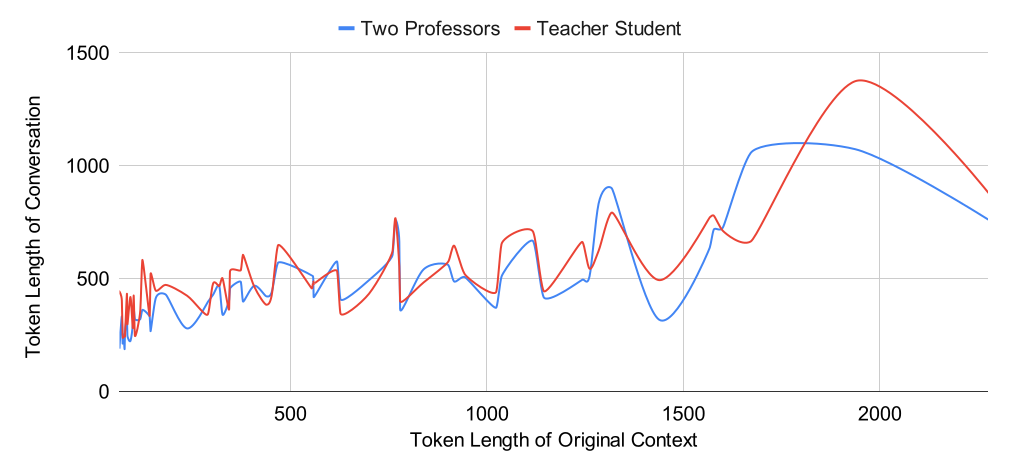
\includegraphics[width=0.8\columnwidth]{figures/context_len.pdf}
  \caption{With increasing context length the generated conversation length decreases!}
  \label{fig:context_length}
\end{figure}





Therefore, we conduct an experiment on 140k samples from the \owm corpus of varying input length to determine the optimal input token length that generates conversations of following characteristics: (1) retains all relevant information from the original context, (2) remains grounded to the source material and (3) enhances the conversation with complementary explanations and reasoning. For each sample, we generate conversations using two prompt (\tp and \ts) and observe the token length of the generations. As depicted in \autoref{fig:context_length}, with increasing input token length (X-axis), the token length of the generated conversation (Y-axis) does not scale up linearly. For example, an input context of 2K tokens results in a conversation that has 1K tokens resulting in a lot of information loss during conversion. Analyzing the \autoref{fig:context_length}, we see that the input token length of 500 can generate conversation that goes beyond 500 tokens meaning that the conversation not only retains information but also adds necessary reasoning  resulting in more tokens. 

% \begin{wrapfigure}{r}{0.5\textwidth}
%     \vspace{-6mm}
%     \centering    
%     \includesvg[width=\textwidth]{figures/context_len.svg}
%     \caption{With increasing context length the generated conversation length decreases!}
%   \label{fig:context_length}
%   % \vspace{-2mm}
% \end{wrapfigure}


\subsection{Conversation Length vs Model Performance}\label{ss:len_vs_acc}


As shown in \autoref{tab:7b_owm_4b}, \textsc{Longest Conversation} achieves the best results among all styles. Since \textsc{Longest Conversation} is curated by selecting the longest dialogue (in terms of token count) from seven conversations for a single context, it raises the question of how dialogue length impacts downstream task accuracy.

\begin{wraptable}[11]{r}{0.5\textwidth}
\centering
\vspace{-6mm}
\resizebox{\textwidth}{!}{% 
\begin{tabular}{@{}lcc@{}}
\toprule
\textbf{Style} &	\textbf{Avg Token Length} &	\textbf{Accuracy (Avg-All)}\\\toprule
\tp &  451.95	& 29.12 \\ 
\tss & 452.17	& 32.65 \\
\ps & 465.29	& 33.38 \\
\ts & 494.03 & 32.87 \\
\intr & 497.21	& 32.12 \\
\deb & 511.90	& 33.11 \\
\lk & 630.23	& 31.74 \\
\textsc{Longest Conversation} & 653.48	& 34.08\\
\toprule
\end{tabular}
}
\caption{\textbf{Conversation Length vs Downstream Task Accuracy:} Conversation length is not correlated with downstream task accuracy.}
\label{tab:len_vs_acc}
\end{wraptable} 

To explore the relationship between dialogue length and accuracy, we measured the average token length of dialogues across all conversational styles, including \textsc{Longest Conversation}. As seen in \autoref{tab:len_vs_acc}, reasoning accuracy does not exhibit a linear correlation with dialogue length. For example, with \ps style we can achieve comparable accuracy to \textsc{Longest Conversation} even when the average token length for \ps is \~ 188 lower than \textsc{Longest Conversation}. This highlights that the conversation length is not the only important factor to attain the maximum gain in reasoning ability. As mentioned in Section \ref{sec:ablations}, the structure and dynamics of the conversations also play a crucial role in maximizing reasoning gains.%The way conversations have been carried out is equally important.




\subsection{Conversation Quality Assessment}\label{ss:quality_assess}


% \paragraph{Conversation Quality Assessment.} \label{ss:quality_assess}
While the conversations generated by the \llm typically appear coherent, there are instances where the conversation fails to preserve the context or lacks grounding to the source material. In some cases, conversations may even be incomplete. Detecting poor-quality generation becomes challenging at scale. To address this, we explore two quality-filtering approaches:

\textbf{Heuristic Filtering.} We employ a simple heuristic based on token length. Given that the input context is limited to a maximum of 500 tokens and split into subcontexts of 500 tokens each to maximize information retention, we discard any generated conversations that fall below 50 tokens. This ensures that minimal information loss is detected early.

\textbf{\llm-based Scoring.} For a more comprehensive assessment, we use an \llm to score the quality of the generated conversations. We introduce four key metrics for evaluation:
\begin{itemize}[leftmargin=*] 
    \item \textbf{Correctness}: Verifies that all information, such as numbers and parameters, is accurately reflected in the conversation.
    \item \textbf{Faithfulness}: Ensures the conversation remains grounded in the context provided.
    \item \textbf{Information Preservation}: Checks whether all relevant facts and knowledge from the original context are retained in the conversation.
    \item \textbf{New Knowledge}: Evaluates whether the conversation introduces additional explanations, reasoning, or definitions not present in the raw input.
\end{itemize}




% \begin{figure}[H]
%   \centering
%   \includesvg[width=0.8\columnwidth]{figures/quality.svg}
%   \caption{LLM tends to rate its generation higher most of the times.}
%   \label{fig:conv_quality}
% \end{figure}


Given a raw context and its corresponding conversation, we ask $\mathcal{M}$ to rate the conversation on a scale of 1 to 5 in each of four metrics, with 1 representing poor quality and 5 representing the best possible conversation. To determine the overall quality, we compute the average score across the metrics and choose conversations with average scores more than or equal to 3. Additionally, we utilize the prompt from the FineWebEdu \citep{penedo2024finewebdatasetsdecantingweb} annotation framework to further check the correlation between two scoring approaches. In \autoref{fig:conv_quality}, we plot the scores for 140K conversations using FineWebEdu metrics and our metrics. It is clearly visible from the figure is that \llm tends to rate its own generation higher almost all the time resulting in a skewed distribution of rating. Around 96\% of conversations are labelled as high quality. However, compared to FineWebEdu, our metric results in less skewed distribution---making our approach more suitable for evaluating synthetic data derived from a seed corpus. % comparison between fineweb metrics and our. our is better

\begin{wrapfigure}{r}{0.5\textwidth}
    % \vspace{-6mm}
    \centering    
    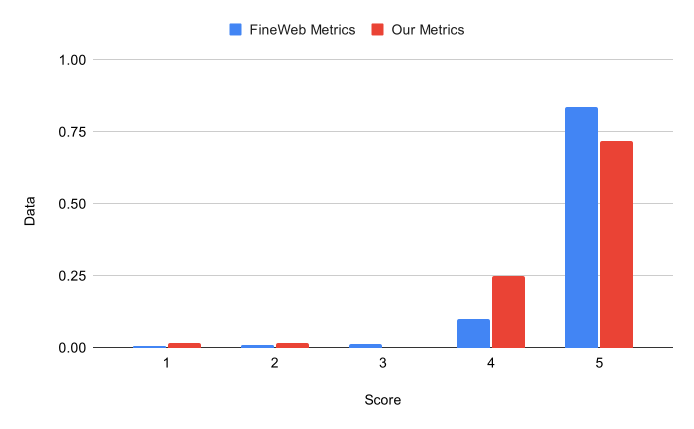
\includegraphics[width=\textwidth]{figures/quality.pdf}
    \caption{LLM tends to rate its generation higher most of the times.}
  \label{fig:conv_quality}
  % \vspace{-2mm}
\end{wrapfigure}

To further investigate, we choose 20 contexts and their corresponding conversations and manually label them on the above four metrics. We later pass these samples to \llm to obtain the quality scores. The correctness and faithfulness metrics were consistently high, with \llm showing a generation correct 96\% of times and human annotators labeling a conversation correct 98\% of times (with spearman correlation between two being 0.82) which validates the quality and reliability of the generated synthetic dialogues.  When comparing the overall human scores with those from the \llm across the four metrics, we observe a weak correlation between two sets (Spearman's $\rho=0.03$) and the reasoning behind them. Human annotators prioritized the information preservation metric, while the \llm often overlooked minor information loss. Additionally, the interpretation of ``New Knowledge" differed between humans and the \llm. Humans valued extra reasoning and explanation as forms of new knowledge, whereas the \llm assigned higher ``New Knowledge" scores to conversations containing out-of-context information that is difficult to verify. Given these differences in the results from human and \llm-based quality filtering, we use simple heuristic filtering in this study and plan to explore other approaches in the future.

\subsection{Compare with \dsm}\label{ss:dsm}

To asses the quality of our data, we run pre-training experiments to compare \ourdata with the recently released \dsm \citep{deepseek-math}. The \dsm approach is iterative. They construct a dataset for binary classification consisting of 500K positive data points randomly sampled from \owm (the seed corpus) and 500K negative data points randomly sampled from \cc. They train a fastText \citep{joulin2016fasttext} classifier on these data which they then use to extract samples from \cc as math content. All \cc domains for which over 10\% of the existing web pages have been extracted are at this point understood to be math-related. URLs which are associated with these domains but which have yet to be collected are manually labeled as math content. The web pages hosted at these addresses are added to the seed corpus and the classifier is retrained. \dsm performs 4 rounds in total resulting in the \dsm Corpus, consisting of some 120B math tokens. They continuously train a partially converged 7B \textsc{DeepSeekCoder-v1.5} model on a 500B token blend to attain the \dsm model and achieve substantial improvement on several math tasks. In contrast, \ourapproach proposes a simple alternative for generating high-quality math data that boosts the mathematical reasoning ability of \llm given access to a small seed corpus. 

As the \dsm dataset is not public, we replicate our previous blend, $\mathcal{D} = \{\mathcal{X}\cup \mathcal{R}_{pt}\}$, where $\mathcal{X} = \{\text{\ourdata-4B} \text{ (conversations of all styles except the \tss one)} \cup \text{\ourdata-14B (\tss conversations)}\}$. We maintain a 2:1 ratio of $\mathcal{X}$ and $\mathcal{R}_{pt}$ in the training blend. Similar to the approach of \dsm, we take a converged \textsc{DeepSeekCoder-v1.5} model as $\mathcal{C}$ --- the unconverged model weights are unpublished as far as we are aware --- and convert the model weights to a format compatible with Megatron-LM, which serves as our training framework, before continuously training for 500B tokens. We use a cosine learning rate schedule with a 19B token linear ramp-up, a maximum learning rate of 3e-4, and a minimum learning rate of 3e-6, and we anneal the learning rate over 500B tokens. We use Adam with parameters $\beta_{1}=0.9$ and $\beta_{2}=0.95$, a weight decay of 0.1, a gradient clipping threshold of 1.0, a sequence length of 4096, and a global batch size of 2304 sequences.

\begin{table*}[ht!]
\begin{center}
\resizebox{\textwidth}{!}{% 
\begin{tabular}{@{}lcccccccc@{}}
\toprule
\textbf{Dataset} & \textbf{Tokens} & \textbf{GSM8K} &\textbf{MATH} & \textbf{\shortstack{MMLU-\\STEM}} & \textbf{MMLU}& 	\textbf{\shortstack{\textsc{General Reasoning}\\(Avg)}} & \textbf{Avg-Math} & \textbf{Avg-All}\\\toprule
\dsm \citep{deepseek-math}& \multirow{3}{*}{500B} & 59.29	& 4.37	& 55.41	& 54.98	& 55.94 & 39.69 & 43.64\\ \cmidrule{3-9}
\ourdata-4B/14B [Combinations$^*$] & & 57.32 &	2.36	&51.95&	56.54	&59.16	& 37.21 &43.84\\ 
% \ourdata-14B [All Conversations] & & 52.46 &	3.24	&54.96&	59.20	&59.38	& 43.57\\ 
\toprule
\end{tabular}
}
\end{center}
\caption{\textbf{\dsm vs All Synthetic Conversations.} A model trained on conversations generated by \ourapproach from a small seed corpus can achieve math accuracy comparable to the \dsm model trained on 120B unique tokens.}
\label{tab:dsm_exp}
\end{table*}

From \autoref{tab:dsm_exp}, we can see that a model trained on conversations which \ourapproach generated given a small seed corpus can attain math accuracies comparable to the \dsm model with access to 120B unique math tokens in its continuous training blend. In fact, we outperform \dsm in \mmlu and general reasoning tasks, reaching higher average accuracy across all tasks. This underscores the quality of \ourapproach generated conversations and signifies the efficacy of \ourapproach in improving mathematical reasoning ability of \llm when the underlying raw data is limited.



In contrast to our prior $\mathcal{C}$, \dsm-7B \llm is a strong math baseline that has been specifically designed for addressing mathematical reasoning ability and surpasses \cite{azerbayev2023llemma}, \cite{gemmateam2024gemmaopenmodelsbased}, \cite{jiang2023mistral7b}, \cite{lewkowycz2022solvingquantitativereasoningproblems}, \cite{javaheripi2023phi}, \cite{dubey2024llama} [8B] base models on diverse math tasks. To evaluate the effectiveness of \ourapproach with stronger pretrained model, we perform an additional experiment, similar to our training setup in Section \ref{ss:training_details} using $\mathcal{C}=$ \dsm-7B. Specifically, we have continuously trained the $\mathcal{C}$ on 500B tokens maintaining a 2:1 ratio of math ($\mathcal{R}$) and 13 CC ($\mathcal{R}_{pt}$) dataset where the total blend is $\mathcal{D} = \{\mathcal{R}\cup \mathcal{R}_{pt}\}$. We conduct two experiments by alternating $\mathcal{R}$ with raw (\owma-14B) and $\mathcal{X}$.

\begin{table*}[ht!]
\begin{center}
\resizebox{\textwidth}{!}{% 
\begin{tabular}{@{}lcccccccc@{}}
\toprule
\textbf{Dataset} & \textbf{Tokens} & \textbf{GSM8K} &\textbf{MATH} & \textbf{\shortstack{MMLU-\\STEM}} & \textbf{MMLU}& 	\textbf{\shortstack{\textsc{General Reasoning}\\(Avg)}} & \textbf{Avg-Math} & \textbf{Avg-All}\\\toprule
\owma-14B & \multirow{3}{*}{500B} & 39.42	& 1.59	& 49.92	& 52.87	& 55.47 & 30.31 & 37.34\\ \cmidrule{3-9}
\ourdata [\textsc{all conversations}] & & 57.32 &	2.36	&51.95&	56.54	&59.16	& 37.21 &43.84\\ 

\toprule
\end{tabular}
}
\end{center}
\caption{\textbf{Training \dsm-7B with Raw Data vs All Synthetic Dialogues.} A strong pretrained \llm continously trained on conversations generated by \ourapproach provides significant boost in math accuracy than the same model trained on raw data---showing the effectiveness of \ourapproach regardless of pretraining model quality.}
\label{tab:dsm_exp_comp}
\end{table*}

As shown in \autoref{tab:dsm_exp_comp}, model trained on \ourdata data shows consistent improvement over model trained on raw data---resulting in 17.90\% gain on \gsm, 6.90\% average improvement across math tasks and 3.43\% average improvement across ten general reasoning tasks. These results further solidifies the effectiveness of \ourapproach regardless of the quality of the pretrained model. 



\subsection{Conversations on Code Tasks}\label{ss:code}



Unlike raw data, conversations tend to break down the context into sub-context and participants exchange their reasoning about the sub-context in a single turn. This feature is particularly useful for mathematical or logical reasoning which require step-by-step reasoning. However, this structure might hurt performance of \llm in domains where sequence of context needs to be preserved such as in codes. To further investigate the impact of conversational data on the coding capabilities of \llm, we conduct an evaluation of models trained on both raw and synthetic data across four established coding benchmarks: HumanEval \citep{chen2021evaluating}, MBPP \citep{austin2021program}, HumanEval+, and MBPP+ \citep{liu2024your}. These benchmarks are specifically designed to assess the model's ability to generate functional code in response to given prompts.


Our results, as presented in \autoref{tab:7b_code}, demonstrate that conversational synthetic data does not enhance coding performance. This is largely due to the way conversations tend to fragment code, wrapping it in natural language and thereby obscuring the intended sequence and logic inherent in programming tasks. Consequently, while conversations may be effective in contexts that benefit from collaborative reasoning, they are not suited for preserving the integrity of code, leading to diminished performance in coding benchmarks. 


\begin{table*}[ht]
\begin{center}
\resizebox{\textwidth}{!}{% 
\begin{tabular}{@{}lcccccc@{}}
\toprule
\textbf{Dataset} & \textbf{Style} & \textbf{HumanEval}        & \textbf{HumanEval+} & \textbf{MBPP (Sanitized)} & \textbf{MBPP+} & \textbf{Avg-All}\\\toprule
\owma-4B &   Raw & 12.20	& 10.98&	23.74 &0.00	&11.73 \\\midrule
Rephrase-\owma-4B & Rephrase &5.49	& 4.27	&20.23	&0.53	&7.63\\\midrule
% & \mawps           & \textbf{69.83}         & 66.83            \\ 
\multirow{9}{*}{\ourdata-4B} %& \textsc{Rephrase} & 5.49	& 4.27	&20.23	&0.53	&7.63\\\cmidrule{2-7}
& \tp & 8.54	& 4.88	&20.62	&0.00	    &8.51\\ 
 & \ts & 13.41	& 9.76	&26.46	&0.26	&12.47\\ 
& \tss & 10.37	& 7.93	&26.07	&0.26	&11.16\\  
& \lk & 10.37	& 8.54	&26.46	&0.79	&11.54\\
& \deb & 11.59	& 9.15	&24.90	&0.26	&11.48\\
& \intr & 7.32	& 4.88	&23.35	&0.26	&8.95\\
& \ps & 9.76	& 9.15	&24.51	&0.26	&10.92\\ \cmidrule{2-7}
& \textsc{Longest Conversation} & 9.15	& 7.32	& 28.40	& 0.53	& 11.35\\
& \textsc{All Conversations} & 12.20	& 9.15	& 28.02	& 0.53	& 12.48\\ \midrule
\owma-4B+\ourdata-4B [1:1] & \multirow{2}{*}{Combination} & 13.41	& 10.98	& 23.35	& 0.00	& 11.94\\ 
\owma-4B+\ourdata-4B [Concat] & & 10.37	& 7.93	& 31.52	& 0.00	& 12.46\\
\toprule
\end{tabular}
}
\end{center}
\caption{\textbf{Results of 7B \llm on Code Tasks:} Conversations and rephrases are ineffective for code benchmarks.}
\label{tab:7b_code}
\end{table*}

Interestingly, we also observe that rephrasing, which resembles raw data more closely in structure, further degrades coding accuracy. Our qualitative analysis of the rephrased documents reveals that the conversation generator (\llama) often removes critical elements such as important tags and code indentation, which are essential for comprehending and executing code correctly. This finding underscores the necessity of designing code-specific prompts that retain the structural components vital for coding tasks. 


\clearpage
\section{Dialogue Examples}\label{ss:conv_example}

% \textbf{\textsc{Raw Text}}
% \begin{tcolorbox}[colback=blue!5!white,colframe=white]
% \# The Truth about Martin Luther King Jr
  
% By Murray Bourne, 09 Jul 2006

% While King's influence on the civil rights movement was overall a Good Thing, I found the King Papers Project interesting, considering he was quite a plagiariser.

% Stanford's own King Encyclopedia gives some background but there is no mention of plagiarism.

% Wikipedia has more on King's authorship issues.
% Was his plagiarism sloppy academic writing or dishonesty? 

% This is the dilemma we face every time we find that a student has copied...

% Footnote: There are some interesting comments on King at Myths of Martin Luther King. Both of these sites have questionable reliability, of course. You have been warned.

% See the 1 Comment below.

% \#\#\# One Comment on "The Truth about Martin Luther King Jr"
% 1. Vinod says:

% If I have seen further, it is by standing on the shoulders of giants.

% \#\#\# Comment Preview

% HTML: You can use simple tags like $<$b$>$, $<$a href=``...''$>$, etc.

% To enter math, you can can either:
% 1. Use simple calculator-like input in the following format (surround your math in backticks, or qq on tablet or phone):

% $a^2 = sqrt(b^2 + c^2)$

% (See more on ASCIIMath syntax); or

% 2. Use simple LaTeX in the following format. Surround your math with \$\$ and \$\$.

% $\$\$\int g dx = \sqrt{\frac{a}{b}}\$\$$

% (This is standard simple LaTeX.)

% NOTE: You can't mix both types of math entry in your comment.

% \end{tcolorbox}

\textbf{\textsc{Raw Text}}
\begin{tcolorbox}[colback=blue!5!white,colframe=white]
\# CAT Quantitative Aptitude Questions | CAT Ratios, Mixtures, Alligations and Averages Questions

\#\#\#\#\#\# CAT Questions | Mixtures and Alligations | Mixtures - Range

The question is from CAT Ratio, Mixtures and Averages. Given the details about two alloys, we need to determine the possible values the weight of an ally can take. CAT exam is known to test on basics rather than high funda ideas. A range of CAT questions can be asked from Ratios and Proportions, Mixtures, Alligations and Averages. Make sure you master the topics. 2IIMs CAT questions bank provides you with CAT questions that can help you gear for CAT Exam CAT 2020.

Question 16: 100 kgs of an alloy of tin and lead in the ratio 1:3 is mixed with x kgs of an alloy of tin and lead in the ratio 3:2. If the overall alloy should contain between 40\% and 50\% tin, what is the range of values x can take?

1. 100 kgs $\leq x \leq$ 200 kgs

2. 80 kgs $\leq x \leq$ 240 kgs

3. 110 kgs $\leq x \leq$ 220 kgs

4. 75 kgs $\leq x \leq$ 250 kgs

\#\# Best CAT Coaching in Chennai

\#\#\#\# CAT Coaching in Chennai - CAT 2020Online Batches Available Now!
\end{tcolorbox}

\vspace{6mm}

% \textbf{\textsc{Synthetic Dialogue [\tp]}}

% \begin{tcolorbox}[colback=red!5!white,colframe=white]
% \textbf{Professor 1:} You know, I was reading about Martin Luther King Jr. and I came across some interesting information. While his influence on the civil rights movement was undoubtedly a good thing, I found out that he was quite a plagiarizer.

% \textbf{Professor 2:} Really? I hadn't heard that about him. What's the source of this information?
% Professor 1: Well, I was looking at the King Papers Project, and it's quite revealing. Stanford's own King Encyclopedia doesn't mention it, but Wikipedia has more on King's authorship issues.

% \textbf{Professor 2:} That's fascinating. Do you think his plagiarism was just sloppy academic writing or outright dishonesty?

% \textbf{Professor 1:} Exactly! That's the dilemma we face every time we find that a student has copied. It's hard to know whether it's just laziness or intentional deception.

% \textbf{Professor 2:} I see what you mean. By the way, I love that quote from Isaac Newton: "If I have seen further, it is by standing on the shoulders of giants." It's a great reminder that we all build on the work of others.

% \textbf{Professor 1:} Ah, nice connection! And yes, it's a great quote. By the way, I also came across some interesting comments on King at Myths of Martin Luther King. Of course, one has to be cautious about the reliability of those sources, but still...

% \textbf{Professor 2:} Absolutely. We always need to approach these kinds of sources with a critical eye. Thanks for sharing this, it's definitely given me something to think about.
% \end{tcolorbox}

\textbf{\textsc{Synthetic Dialogue [\tp]}}

\begin{tcolorbox}[colback=red!5!white,colframe=white]
\textbf{Professor 1:} Good morning, colleague. I'd like to discuss a question from CAT Ratio, Mixtures, and Averages. It's about two alloys of tin and lead, and we need to determine the possible values of the weight of an alloy.

\textbf{Professor 2:} Ah, yes. I'm familiar with this type of question. It's a classic example of Mixtures and Alligations. Please go ahead and share the details of the question.

\textbf{Professor 1:} We have 100 kgs of an alloy of tin and lead in the ratio 1:3, which means it has 25 kgs of tin and 75 kgs of lead. This alloy is mixed with x kgs of another alloy of tin and lead in the ratio 3:2. The overall alloy should contain between 40\% and 50\% tin. We need to find the range of values x can take.

\textbf{Professor 2:} That's a great problem. We can start by analyzing the second alloy. If it has a ratio of 3:2, that means it has 3x/5 kgs of tin and 2x/5 kgs of lead, with a total weight of x kgs.

\textbf{Professor 1:} Exactly. Now, when we mix these two alloys, how does the mixture change? We need to find the overall percentage of tin in the resulting alloy.

\textbf{Professor 2:} Right. Let's think about it. If the overall alloy should contain between 40\% and 50\% tin, what does that imply about the range of values x can take?

\textbf{Professor 1:} That's the key question. If we can determine the range of x, we can answer the question. Do you think it's possible to narrow down the options to one of the given choices?

\textbf{Professor 2:} Yes, I think so. Let's analyze the options. We have 1. 100 kgs $\leq x \leq$ 200 kgs, 2. 80 kgs $\leq x \leq$ 240 kgs, 3. 110 kgs $\leq x \leq$ 220 kgs, and 4. 75 kgs $\leq x \leq 250$ kgs. Which one do you think is the correct answer?

\textbf{Professor 1:} Well, after analyzing the problem, I think the correct answer is option 2: 80 kgs $\leq x \leq$ 240 kgs. What do you think?

\textbf{Professor 2:} I agree with you. The correct answer is indeed option 2. Well done! This question is a great example of how CAT exam tests our understanding of basics rather than high-funda ideas.
\end{tcolorbox}


\clearpage

\textbf{\textsc{Raw Text}}
\begin{tcolorbox}[colback=blue!5!white,colframe=white]
?

Free Version

Moderate

\# Interpretation of Equilibrium from Graph of Concentration vs Time

CHEM-NWU9LE

Consider the graph below of a chemical reaction observing the concentration of two chemical species with time.

Which species is the reactant?
\$\$

Which species is the product?

\$\$

At what region does the solution appear to be in equilibrium?
\$\$

What is the $K_c$ for the reaction?
\end{tcolorbox}

\vspace{6mm}

\textbf{\textsc{Synthetic Dialogue [\ts]}}

\begin{tcolorbox}[colback=red!5!white,colframe=white]

\textbf{Student:} Hi, teacher. I'm having trouble understanding this graph of a chemical reaction. Can you help me?

\textbf{Teacher:} Of course! What's your first question about the graph?

\textbf{Student:} Okay, so which species is the reactant?

\textbf{Teacher:} Let's take a look at the graph. The species whose concentration is decreasing with time is the reactant. Can you identify which one that is?

\textbf{Student:} Ah, I think it's... (looks at the graph) ...the one whose concentration starts high and decreases.

\textbf{Teacher:} That's correct! The reactant is the species whose concentration starts high and decreases with time. Now, what's your next question?

\textbf{Student:} Which species is the product?

\textbf{Teacher:} Good question! The product is the species whose concentration starts low and increases with time. Can you identify which one that is?

\textbf{Student:} Yeah, I think it's... (looks at the graph) ...the one whose concentration starts low and increases.

\textbf{Teacher:} That's right! The product is the species whose concentration starts low and increases with time. Now, what's your next question?

\textbf{Student:} At what region does the solution appear to be in equilibrium?

\textbf{Teacher:} Look at the graph again. At what point does the concentration of both species seem to be constant, not changing with time?

\textbf{Student:} Hmm... I think it's... (looks at the graph) ...after a certain time, when the lines are flat.

\textbf{Teacher:} Exactly! The solution appears to be in equilibrium when the concentration of both species is constant, which is after a certain time when the lines are flat. Now, what's your next question?

\textbf{Student:} What is the Kc for the reaction?

\textbf{Teacher:} Unfortunately, the graph doesn't provide enough information to calculate the Kc value. We would need more data or information about the reaction to determine the equilibrium constant, Kc.

\textbf{Student:} Okay, I think I understand now. Thank you for your help!
\end{tcolorbox}

\clearpage

\textbf{\textsc{Raw Text}}
\begin{tcolorbox}[colback=blue!5!white,colframe=white]
    
    What's the probability that: The person is not age 18 to 34 and does not own an iPhone?
    
    The presidential election is coming.
    
    Five survey companies (A, B, C, D, and E) are doing survey to forecast whether or not the Republican candidate will win the election.
    
    Each company randomly selects a sample size between 1000 and 1500 people.
    
    All of these five companies interview people over the phone during Tuesday and Wednesday.
    
    The interviewee will be asked if he or she is 18 years old or above and U.S. citizen who are registered to vote. If yes, the interviewee will be further asked: will you vote for the Republican candidate?
    
    On Thursday morning, these five companies announce their survey sample and results at the same time on the newspapers.
    
    The results show that a\% (from A), b\% (from B), c\% (from C), d\% (from D), and e\% (from E) will support the Republican candidate.
    
    The margin of error is plus/minus 3\% for all results.
    
    Suppose that $c{>}{a}{>}{d}{>}{e}{>}{b}$.
    When you see these results from the newspapers, can you exactly identify which result(s) is (are) not reliable and not accurate?
    
    That is, can you identify which estimation interval(s) does (do) not include the true population proportion?
    
    If you can, explain why you can, if no, explain why you cannot and what information you need to identify.
    
    Discuss and explain your reasons. You must provide your statistical analysis and reasons.
\end{tcolorbox}

% \clearpage

\textbf{\textsc{Synthetic Dialogue [\tss]}}

\begin{tcolorbox}[enhanced jigsaw,breakable,pad at break*=1mm,colback=red!5!white,colframe=white]
\textbf{**Turn 1**}

Alex: Hey Ben, have you started working on our assignment about the presidential election survey?

Ben: Yeah, I've been going over the context. It seems like we need to identify which survey result is not reliable and accurate.

Alex: Exactly! Let's break it down. We have five survey companies, A, B, C, D, and E, each with a sample size between 1000 and 1500 people.

Ben: Right, and they all have a margin of error of plus/minus 3\%.



\textbf{**Turn 2**}

Alex: Okay, so we're given that c $>$ a $>$ d $>$ e $>$ b. What does this tell us?

Ben: It tells us the order of the proportions of people who will support the Republican candidate according to each survey company.

Alex: That's right. And since the margin of error is the same for all companies, we can assume that the true population proportion should lie within a similar range for all companies.



\textbf{**Turn 3**}

Ben: But wait, if the true population proportion lies within a similar range, then shouldn't all the estimation intervals overlap?

Alex: Exactly! If the estimation intervals don't overlap, it means that at least one of them is not reliable and accurate.

Ben: So, we need to check if the intervals overlap. How do we do that?



\textbf{**Turn 4**}

Alex: Let's calculate the estimation intervals for each company. For company A, it's a\% $\pm$ 3\%, and similarly for the others.

Ben: Okay, got it. So, we have a\% $\pm$ 3\%, b\% $\pm$ 3\%, c\% $\pm$ 3\%, d\% $\pm$ 3\%, and e\% $\pm$ 3\%.

Alex: Now, let's check if these intervals overlap. Since c $>$ a $>$ d $>$ e $>$ b, the interval for company C should be the highest, and the interval for company B should be the lowest.



\textbf{**Turn 5**}

Ben: I see what you're getting at. If the intervals overlap, then the highest value of the lowest interval (company B) should be greater than or equal to the lowest value of the highest interval (company C).

Alex: That's right! If that's not the case, then we know that at least one of the intervals is not reliable and accurate.

Ben: Let's plug in some numbers and see if we can identify which one is not reliable.



\textbf{**Turn 6**}

Alex: Alright, let's say the results are a = 45\%, b = 38\%, c = 50\%, d = 42\%, and e = 40\%. Can we identify which one is not reliable?

Ben: Let's calculate the estimation intervals... (calculates)...and check if they overlap.

Alex: (checks the calculations) Ah, look at that! The interval for company B (38\% $\pm$ 3\%) doesn't overlap with the interval for company C (50\% $\pm$ 3\%).

Ben: That means company B's result is not reliable and accurate!



\textbf{**Turn 7**}

Ben: But why can't we identify the other unreliable results, if any?

Alex: That's because we only have the relative order of the proportions, not the exact values. We need more information to identify other unreliable results, if any.

Ben: I see. So, we can only identify company B's result as not reliable and accurate, but we can't say for sure about the others.

Alex: That's correct. We've done our best with the given information.
\end{tcolorbox}

\clearpage


\textbf{\textsc{Raw Text}}
\begin{tcolorbox}[colback=blue!5!white,colframe=white]
  \# Decimal to Percent Calculator.
  
  The calculator will convert decimal into percent, with steps shown.
  
  If the calculator did not compute something or you have identified an error, or you have a suggestion/feedback, please write it in the comments below.
  
  Convert $1.4$ into decimal.  \#\# Solution From the converting decimal to percent note, we know that to obtain a percent, we need to multiply a decimal by $100$.
  
  But multiplying by $100$is equivalent to moving a decimal point $2$ positions to the right.
\end{tcolorbox}

\vspace{6mm}

\textbf{\textsc{Synthetic Dialogue [\lk]}}

\begin{tcolorbox}[colback=red!5!white,colframe=white]
    \textbf{**Turn 1**}
    
    Layman: Hi, I'm not sure what this calculator does. Can you explain it to me?
    
    Me: This calculator converts decimals into percents. It shows the steps to do the conversion.
    
    \textbf{**Turn 2**}
    
    Layman: Okay, got it. So what's the problem we're trying to solve?
    
    Me: We're trying to convert 1.4 into a percent.
    
    \textbf{**Turn 3**}
    
    Layman: How do we do that? Is there a formula or something?
    
    Me: Yes, there is. According to the note on converting decimal to percent, we need to multiply the decimal by 100 to obtain a percent.
    
    
    \textbf{**Turn 4**}
    
    Layman: Why do we need to multiply by 100? What's the logic behind it?
    
    Me: Well, I'm not sure about the logic, but the note says that's what we need to do. But I can tell you that multiplying by 100 is equivalent to moving the decimal point 2 positions to the right.
    
    \textbf{**Turn 5**}
    
    Layman: What do you mean by moving the decimal point 2 positions to the right? Can you explain that?
    
    Me: Sure. When you multiply a number by 100, the decimal point shifts 2 places to the right. For example, if you have 1.4 and you multiply it by 100, the decimal point will move 2 places to the right, making it 140.
    
    \textbf{**Turn 6**}
    
    Layman: Ah, I think I understand now. So, if we multiply 1.4 by 100, what do we get?
    
    Me: That's right! If we multiply 1.4 by 100, we get 140. And that's the equivalent percent value of the decimal 1.4.
\end{tcolorbox}

\clearpage


\textbf{\textsc{Raw Text}}
\begin{tcolorbox}[colback=blue!5!white,colframe=white]
Try to finish the derivation and see how it applies to the sum you're trying to compute. Sorry if this is hard to understand.

7. Jun 14, 2009

\#\#\# jgens

Cyosis, why would he/she use the sum for the first n natural numbers when his sum asks for odd natural numbers only?

8. Jun 14, 2009

\#\#\# Cyosis

If you know the sum for the first n natural numbers you can quickly solve the sum for the first odd numbers. Had he known it, it would have been the easiest way to calculate the sum he's interested in.

9. Jun 14, 2009

\#\#\# Manchot

The story is that a six-year-old Gauss was told by his teacher to add the numbers 1 to 100 as a form of busywork. In seconds, he came up with the answer, much to his teacher's surprise. What he did was notice that since 1+100=101, 2+99=101, 3+98=101, etc., the sum becomes a simple multiplication: there are 50 of the above \"pairs,\" so the sum is just 50*101 = 5050. Anyway, that's the intuition behind the identity that Cyosis posted. You can pretty much use the exact same intuition.

10. Jun 14, 2009

\#\#\# gabrielh

Okay thanks, I get it now.


11. Jun 14, 2009
\end{tcolorbox}

\vspace{6mm}


\textbf{\textsc{Synthetic Dialogue [\deb]}}

\begin{tcolorbox}[colback=red!5!white,colframe=white]
\textbf{jgens}: I don't understand why Cyosis suggested using the sum of the first n natural numbers to solve the problem. The original problem asks for the sum of the first odd natural numbers, not all natural numbers.

\textbf{Cyosis}: I see what jgens is saying, but I think my approach is still valid. If you know the sum of the first n natural numbers, you can easily derive the sum of the first odd natural numbers. It's actually the easiest way to calculate the sum.

\textbf{Manchot}: I think I can help clarify things. The story about Gauss adding numbers from 1 to 100 is relevant here. He noticed that 1+100=101, 2+99=101, and so on, which makes the sum a simple multiplication problem. There are 50 such pairs, so the sum is 50*101 = 5050. This is the intuition behind Cyosis' suggestion.

\textbf{jgens}L I see what Manchot is saying, but I'm still not convinced. How does this story about Gauss relate to the sum of odd natural numbers?

\textbf{Cyosis}: Well, jgens, the same intuition applies here. We can use a similar pairing method to calculate the sum of odd natural numbers. It's not a direct application, but the principle is the same.

\textbf{gabrielh}: I think I'm starting to get it now. So, we can use the sum of the first n natural numbers as a stepping stone to calculate the sum of the first odd natural numbers, and the Gauss story provides the intuition behind this approach.

\textbf{Manchot}: Exactly, gabrielh! That's the idea. By understanding the sum of the first n natural numbers, we can derive the sum of the first odd natural numbers using a similar method.

\textbf{Cyosis}: I'm glad we could clarify things. The key is to recognize that the sum of the first n natural numbers is a more general problem that can be used to solve the more specific problem of the sum of the first odd natural numbers.
\end{tcolorbox}

\clearpage

\textbf{\textsc{Raw Text}}
\begin{tcolorbox}[colback=blue!5!white,colframe=white]

The Cryptographic Lens

Shafi Goldwasser - Colloquium Lecture - POSTPONED!

Tuesday, 21.10.2014, 14:30

Room 337-8 Taub Bld.

...

ceClub: A Centralized \"Zero-Queue\" Network Architecture

Jonathan Perry (MIT, CSAIL)

Monday, 06.10.2014, 11:00

EE Meyer Building 861

Current datacenter networks inherit the principles that went into the design of the Internet, where packet transmission and path selection decisions are distributed among the endpoints and routers. Instead, we propose that each sender should delegate control—to a centralized arbiter—of when each packet should be transmitted and what path it should follow. Fastpass is a datacenter network architecture built using this principle. Fastpass incorporates two fast algorit...


Parameterized Automata Constructions and Their Applications

Ran Ben-Basat

Monday, 22.09.2014, 15:30

Taub 701

Parameterization is a useful tool for handling NP-hard problems in the real world. It aims to reduce the running times of algorithms for such problems, by confining the combinatorial explosion to some parameter k. As this parameter is often significantly smaller than the input size, it allows to develop practical algorithms for non-trivial classes of instances for these problems. In this talk we present a novel framework for developing parameterized algorithms, using construction...

Observing the Observers: Social Context Analysis Using Computer Vision

Meir Cohen

Wednesday, 10.09.2014, 12:00

Taub 601

It is quite common that multiple human observers attend to a single point of interest.

Mutual awareness activity (MAWA) refers to the dynamic of this social phenomena.

A peak of a MAWA is known as a mutual awareness event (MAWE) and can be interpreted as a \"buzz\" event, which draws the attention of many observers.

A preferred way to monitor those social phenomenon is with a camera that captures the human observers while they observe the activity in the scene.

Our work studies the ...
\end{tcolorbox}

\vspace{6mm}

\textbf{\textsc{Synthetic Dialogue [\intr]}}

\begin{tcolorbox}[enhanced jigsaw,breakable,pad at break*=1mm, colback=red!5!white,colframe=white]

\textbf{Subject Matter Expert:} Unfortunately, the lecture was postponed, so we don't have any information about the specific topic she was going to cover. However, the title of the lecture was \"The Cryptographic Lens,\" which suggests that it might have been related to cryptography and its applications.

\textbf{Interviewer:} That's a shame it was postponed. Moving on, let's talk about the ceClub lecture by Jonathan Perry from MIT, CSAIL. Can you summarize the main idea behind his proposed datacenter network architecture, Fastpass?


\textbf{Subject Matter Expert:} Yes, certainly. Jonathan Perry proposed a centralized \"zero-queue\" network architecture called Fastpass, which is a departure from the traditional distributed approach used in Internet design. In Fastpass, each sender delegates control to a centralized arbiter, which decides when each packet should be transmitted and what path it should follow. This approach aims to improve the efficiency of datacenter networks.

\textbf{Interviewer:} That's fascinating. What can you tell me about the talk by Ran Ben-Basat on parameterized automata constructions and their applications?


\textbf{Subject Matter Expert:} Ran Ben-Basat discussed the concept of parameterization, which is a useful tool for handling NP-hard problems in the real world. The idea is to reduce the running times of algorithms for these problems by confining the combinatorial explosion to some parameter k. He presented a novel framework for developing parameterized algorithms using construction-based methods.


\textbf{Interviewer:} I see. Now, let's switch gears and talk about the lecture by Meir Cohen on social context analysis using computer vision. Can you explain what mutual awareness activity (MAWA) and mutual awareness event (MAWE) refer to in this context?


\textbf{Subject Matter Expert:} Yes. Mutual awareness activity (MAWA) refers to the dynamic of multiple human observers attending to a single point of interest. A peak of this activity is known as a mutual awareness event (MAWE), which can be interpreted as a \"buzz\" event that draws the attention of many observers. Meir Cohen's work focuses on monitoring and analyzing these social phenomena using computer vision, specifically by capturing the human observers with a camera while they observe the activity in the scene.

\end{tcolorbox}


\clearpage

\textbf{\textsc{Raw Text}}
\begin{tcolorbox}[colback=blue!5!white,colframe=white]
Note: At section X = 12 m, the speed is close to 1.5 m / s Thus for a return trip of 2x20m = 40 m to return to the profile X = 14m, the wave takes 27 s. Thus, the graph of Figure. 11 is located before the (eventual) reflected wave coming from the absorbing upstream boundary, which can disturb the sensors.

\#\# Comparative analysis of records

We have exploited some of the tests in a transversal manner, to identify particular behaviors of the surface waves:

• impact of the variation of the amplitude for several tests characterized by the same parameters but with roughnesses, or geometries either uniform, or linear

• impact of the change in the period

• impact of the variation of the initial amplitude

• comparison for the same test carried out in uniform or converging section

• impact of roughness variation


\#\#\# Impact of the variation of the amplitude for several tests with the same parameters

We have compared several tests characterized by D70, by Ab absorbing boundary conditions and for the same period T5. These are tests D70A5T5, D70A2T2 and D70A5T7 in RoAbUn, SmAbCo and SmAbUn conditions

Figure 16 Figure 17 Figure 18

• Figure 16: amplitudes variations for the 3 runs are increasing according to the slope, which is in accordance with the theory.

• Figure 17: the initial amplitudes of the waves generated by the wave maker are not always well respected: all the curves of the same diagram should start from the same point to X = 0

• Figure 18: there is a sharp change in amplitude at the arrival at the top of the slope.
\end{tcolorbox}


% \vspace{6mm}

\textbf{\textsc{Synthetic Dialogue [\ps]}}

\begin{tcolorbox}[colback=red!5!white,colframe=white]

\textbf{User:} Hi, I'm analyzing some data on surface waves and I'd like to discuss some observations with you. Can you help me understand the impact of varying amplitude on surface waves?

\textbf{AI Assistant:} I'd be happy to help. From the context, I see that you have several tests with the same parameters but different amplitudes. Specifically, you have tests D70A5T5, D70A2T2, and D70A5T7 in RoAbUn, SmAbCo, and SmAbUn conditions. What would you like to know about these tests?

\textbf{User:} Yes, that's correct. I'm looking at Figures 16, 17, and 18. Can you explain what's happening in Figure 16?

\textbf{AI Assistant:} In Figure 16, the amplitudes of the waves are increasing according to the slope, which is consistent with theoretical expectations. This suggests that the amplitude of the wave is directly related to the slope of the surface.

\textbf{User:} That makes sense. But what about Figure 17? The initial amplitudes of the waves generated by the wave maker don't seem to be consistent.

\textbf{AI Assistant:} That's a good observation. Yes, the initial amplitudes of the waves don't start from the same point at X = 0, which is unexpected. This could be an issue with the wave maker or the experimental setup.

\textbf{User:} Okay, got it. And what about Figure 18? There seems to be a sudden change in amplitude at the top of the slope.

\textbf{AI Assistant:} Yes, that's correct. Figure 18 shows a sharp change in amplitude at the arrival at the top of the slope. This could be due to the interaction between the wave and the slope, causing a sudden increase or decrease in amplitude.

\textbf{User:} That's helpful. So, what can we conclude about the impact of varying amplitude on surface waves?

\textbf{AI Assistant:} Based on these figures, it seems that the amplitude of the wave is directly related to the slope of the surface, and changes in amplitude can affect the behavior of the wave. However, we also need to consider the potential issues with the wave maker or experimental setup that may be affecting the results.

\textbf{User:} Okay, that's a good summary. Thanks for your help in analyzing these figures!

\end{tcolorbox}


% \subsection{Continuous Training of Model with Larger Token Budget}